%% Bachelor Thesis Template of Xidian Uniersity
%%   for using XDBAthesis package with LaTeX
%%
%% Created by Xue-Jilong(xuejilong@gmail.com)
%%
%% template.tex v0.1, 2011/03/21


\documentclass[xetex,adobefonts,master]{XDBAthesis}
% 选项说明:
% dvipdfm  使用 dvipdfm(x) 生成最终的 PDF 文档 (缺省设置)
% dvips    使用 dvips 生成最终的 PS 文档
% pdftex   使用 pdfLaTeX 生成最终的 PDF 文档
% xetex    使用 XeLaTeX 生成 PD F文档
% adobefonts 使用 Adobe 中文字体
% winfonts 使用 Windows 中文字体
% master   用于生成硕士学位论文

% 图形文件的搜索路径
\graphicspath{{chapter-utf8/}{figures/}}

\begin{document}
%%----------------- 封面部分 ----------------- %%
    \schoolnumber{1203121619}
    \title{基于压缩后缀数组的短读比对算法}{}   %%题目超过14个字把剩下的放到第二个空
    \entitle{A Short Read Aligment Algorithm with}{ Compressed Suffix Array}   %%题目超过14个字把剩下的放到第二个空
    \major{计算机软件与理论}
    \author{李双江}
    \advisor{霍红卫}
    \date{二〇一四年十月}
    \majorclass{工科}

    \identifier{007}
    \classnumber{1-1(分类号)}
    \classification{公开}
    \maketitle

%%----------------- 前言部分 ----------------- %%
    \frontmatter
    \pagestyle{empty}
    \begin{center}
\heiti\zihao{3}西安电子科技大学\\[5mm]
	学位论文独创性(或创新性)声明
\end{center}\vspace{1cm}

\songti\zihao{-4}秉承学校严谨的学分和优良的科学道德,本人声明所呈交的论文是我个人
在导师指导下进行的研究工作及取得的研究成果。尽我所知,除了文中特别加以标注
和致谢中所罗列的内容以外,论文中不包含其他人已经发表或撰写过的研究成果;
也不包含为获得西安电子科技大学或其它教育机构的学位或证书而使用过的材
料。与我一同工作的同志对本研究所做的任何贡献均已在论文中做了明确的说明
并表示了谢意。

申请学位论文与资料若有不实之处,本人承担一切相关的法律责任。\\[3mm]

	本人签名:\rule{2.6cm}{0.75pt}  \hspace{3cm}  日期\rule{3cm}{0.75pt}\\[2cm]
	
\begin{center}
\heiti\zihao{3}西安电子科技大学\\[5mm]
	关于论文使用授权的说明
\end{center}\vspace{1cm}

\songti\zihao{-4}本人完全了解西安电子科技大学有关保留和使用学位论文的规定,即:研究
生在校攻读学位期间论文工作的知识产权单位属西安电子科技大学。学校有权保
留送交论文的复印件,允许查阅和借阅论文;学校可以公布论文的全部或部分内
容,可以允许采用影印、缩印或其它复制手段保存论文。同时本人保证,毕业后
结合学位论文研究课题再撰写的文章一律署名单位为西安电子科技大学。(保密的
论文在解密后遵守此规定)

本学位论文属于保密,在\rule{6mm}{0.75pt}年解密后适用本授权书。\\[3mm]

	本人签名:\rule{2.6cm}{0.75pt}  \hspace{3cm}  日期\rule{3cm}{0.75pt}\\[3mm]

	导师签名:\rule{2.6cm}{0.75pt}  \hspace{3cm}  日期\rule{3cm}{0.75pt}           

    
\begin{abstract}

新一代基因测序技术(NGS)的出现使得测序成本飞速下降,随之而来的是大量的短读
需要更快速准确的比对程序来处理。第一代基于散列表技术的序列比对算法如MAQ等
能够快速准确的完成比对工作,但其不支持gap比对的特性使得在短读序列(short reads)
过长导致indel出现频繁时,比对的精度也随之下降。另一方面,近年来压缩索引(BWT,CSA,FM-index)
领域的相关研究使得在较小内存中索引人类基因组这样的大规模序列成为可能。这导致
近年来出现了很多基于压缩索引的短读比对算法,如BWA,Bowtie等。本文提出了一种基于压
缩后缀数组和后向搜索实现的近似匹配的算法来实现短读比对,在比对时间和空间以及比对
精度上都取得了很好的效果。

本文提出并实现的基于压缩后缀数组的短读比对算法(CSAA),采用了压缩后缀数组
的后向搜索来做近似匹配。通过引入搜索树,CSAA支持完全的gap比对。另一方面
CSAA在搜索树上使用了一种类似堆的优先堆数据结构,使得搜索树上的搜索空间大大
下降,而且每一次的搜索方向都能保证是最优的。最后结合罚分机制以及$difference$
距离,定义seed等方法,进一步降低搜索空间,提高CSAA的比对速度和精度。

CSAA的高效体现在两个方面,一是空间高效的索引方法。二是高效的近似匹配方法,包括
后向搜索,seed策略和多线程比对技术的利用。本文采用了增量法进行压缩后缀数组索引
的构建,从而跳过后缀数组的构建,降低了对内存的需求。而在比对时,seed的引入使得
在比对短读的前几十个核苷酸就可以放弃大部分无效的搜索方向。多个短读比对的相互
独立使得并行化成为可能,CSAA使用多线程时可以获得数倍的加速优势,可以根据计算
机的cpu核数指定多个线程,以取得最优的比对速度。


CSAA支持单端和双端序列比对,以Fastq格式输入,输出为标准的SAM(Sequence Alignment Map)
格式。

\keywords{短读比对,序列比对,压缩索引,压缩后缀数组}

\end{abstract}

\begin{englishabstract}

\setlength\parindent{0em}

\vspace{2ex}
Nowadays,decreasing cost and better accessibility of next generation sequencing methods
have produced a large amount of short reads whic is calling for the development of fast
and accurate read alignment programs.A first generation of hash-table based methods has
been developed,including MAQ,which is accurate,feature rich and fast enough to align short
reads from a single individual.However,MAQ does not support gapped alignment of longer reads
where indels may occur frequently.On the other hand,recent experimental studies on compressed
indexs(BWT,CSA,FM-index)have confirmed their practivality for indexing very long strings such
as human genome in the main memory,and many alignment method based on compressed index have
been developed,for example,BWA.In this paper we show how to build a software called CSAA that
exploits a CSA index of reference sequence,and perform well on alignment speed and accuration.

\vspace{2ex}
We proposed and implemented Compresses Suffix Array Alignment(CSAA),a new short read alignment
tool that is bases on backward search with compressed suffix array,to align short reads to a
large reference such as human genome.CSAA use a seach tree on multiple proximate sequences to
support mismatch and gapped alignment,CSAA also introduced a heap like structure to decrease
search space on seach tree.Finally,with the help of penalty strategy and seed,CSAA achieved
similar accuracy and faster speed than MAQ.


\vspace{2ex}
CSAA has two advantage. On one hand,increment CSA construction algorithm has beeb used in
CSAA,which directly construct CSA without SA,and use little memory to classic CSA construction algorithm.
On the other hand,CSAA used seed strategy to speed up alignment,which can drop most of invalid
seach direction when aligning the first dozons of nucleotides of a read.Lastly,indpendency of
every short read's aligment makes parallel aligning avaliable.CSAA speed up efficiently by
adopting multi-thread.

\vspace{2ex}
CSAA supports single-end and pair-end mapping with Fastq as input format and SAM(Sequence Alignment Map)
as output format.CSAA also support multi-thread running on a multi-core machine to get a faster
alignment speed.


\englishkeywords{short reads alignment, DNA sequence alignment, comressed index, compress suffix array}

\end{englishabstract}


    \tableofcontents

%%----------------- 正文部分 ----------------- %%
    \mainmatter
    \pagestyle{content}
    \chapter{绪论}
\label{chap:introduction}

\section{研究背景及意义}

DNA(脱氧核糖核酸)是生物遗传信息的载体,其双螺旋结构的两个链互相补充,构成稳定结构。其中每个链都含有完备的遗传信息,这些
遗传信息体现在构成DNA链的四种碱基——腺嘌呤(A),胸腺嘧啶(T),鸟嘌呤(C)和胞嘧啶(G)的排列顺序上。在现代生物学研究中,
为分析DNA的遗传表达等特性,需要特定对物种DNA进行测序。早期的sanger测序作为第一代测序手段在人类基因组计划中起到了巨大的作用。

随着生物学,医学等相关科学的发展,新的DNA测序技术不断涌现,其中,以Illumina/Solexa为代表的NGS(Next-Generation Sequencing technologies)
技术以其低廉的测序成本和便捷快速的特点成为当前的主流DNA测序技术。基于这一新技术实现的测序机器每台工作一天就能产生数十亿的
短读序列(short reads)\cite{metzker2009sequencing}。NGS测序技术一般应用于两类测试场景,重测序(Resequencing)
和从头测序(de novo sequencing),这也对应着产生了DNA分析领域的两个最核心的研究问题:比对(alignment)和重组(assembly)。
若测序的目标物种的基因序列之前还从未被测序过,那么从头测序就是研究的第一步,这需要关注把短读以最优方式连接起来。若测序目标
物种已经完成了测序,那么重测序关注的问题是如何把短读序列映射到已知的同物种基因组上,从而分析同源生物的个体基因差异,这个过
程就是本文关注短读比对(short read alignment)。由于每一次测序实验都会得到大量的短读(short reads)序列(5亿到20亿个),同时生物
个体基因之间的差异会导致基因序列存在差异,短读映射面临着基因的近似比对和快速高效比对两个难题。本文即提出一种基于压缩后缀
数组索引算法的快速高效比对算法来解决这两个问题。

重测序得到的短读序列中每一个短读一般不超过1000个碱基(大多数情况下都是20到100个碱基的长度),但一次测序实验中短读数量都
会超过一千万个。参考序列是已经经过准确测序,重组后的已知基因组序列,比如人类基因组序列就是合并出来的总长达2.8G的DNA序列。
出于医疗,身份鉴别等原因会对某个具体的人进行再次DNA测序,这就是DNA重测序,此时测序得到的大量短读序列分析的第一步就是把
这些短读映射到参考序列上,对人类而言,大多都是映射到人类基因组序列上,也可以映射到一个人工合成的参考序列上。映射的过程是
对每一个短读在参考序列上查找的过程,即要在参考序列上找到一个合适的位置,使得从这个位置开始,短读是参考序列的一个子串。

综上所述,短读序列的比对问题可以抽象为一个模式查找问题:给定一个共有$m$个模式的模式集合$P=\{P_1,P_2\ldots P_m\}$,每个
模式的长度已知分别为$l_1,l_2\ldots l_m$,已知一个长为$n$的参考序列$T$,求得一个集合$S=\{s_1,s_2\ldots s_n\}$使
得$P_i=T[s_i\ldots s_i+l_i-1]$。这个查找的过程即为短读到参考序列的比对映射。其中参考序列$T$和短读序列$P_i$都是由DNA测序
中常用的碱基字符$\{A,T,C,G,N\}$构成的。

\section{研究现状}
为实现快速且准确的短读序列映射,近年来出现了很多比对算法。所有这些算法都可以分为两类,一类是通过对短读序列使用散列表等方法建
立短读序列的索引,之后遍历整个参考序列。另一类是为参考序列建立索引,之后再对每个短读进行独立的比对。

第一类比对算法的代表是MAQ,ZOOM,SHRiMP等。MAQ\cite{li2008mapping}基于散列技术,结合短读中每一个核苷酸的测序质量分数,实现了
无空位(ungapped)比对。ZOOM\cite{lin2008zoom}使用了space seeds技术,提高了比对的精确率。而SHRiMP\cite{rumble2009shrimp}则结合space seeds''
和smith-waterman算法得到了更高的精确率。

第二类算法为参考序列建立索引,通过索引后的数据可以实现快速的比对。如SOAP,WHAM,BFAST等。SOAP\cite{li2008soap}使用seeds技术
和一个散列查询表加速比对,且可以处理较少的空位比对。WHAM\cite{li2012wham}对参考序列建立散列表,先通过散列表查找潜在的比对
位置,再进一步比对确定最终结果。BFAST\cite{homer2009bfast}则通过
为参考序列建立多个索引来提高精确度。这几种方法使用的索引方法都需要很大的内存空间,所以比对时空间需求很大,尤其是在用类基因
组这样的较大序列作为参考序列时。在第二类方法中以SOAP2,Bowtie,BWA为代表的基于BW变换(Burrows-Wheeler transform,BWT)\cite{ferragina2005indexing}来创建参考序列
索引的方法具有很大的空间优势。Bowtie\cite{langmead2009ultrafast}使用BWT建立索引,采用回溯递归
的搜索方法,再结合双端搜索实现了高速,空间高效的比对,是目前最快的比对软件之一,但缺陷是不能实现空位(gap)比对。BWA\cite{li2009fast}
也是基于BWT的一种比对算法,比对速度较Bowtie慢,但可实现空位比对。SOAP2\cite{li2009soap2}使用了bidirectional BWT来建立参考序列
的索引,比对速度和Bowtie相当。基于BWT的这些方法都使用了后向搜索方法\cite{lippert2005space}来加速查询。后向搜索可以在$O(m)$时间内实
现长为$m$的字符串的计数查询,以及$O(m\log n)$时间复杂度的query查询。利用后向搜索的性质,Bowtie实现了基于
回溯法的非精确匹配算法,而BWA则采用前缀树搜索的方法实现非精确匹配。在实现非精确匹配的基础上,加上一些打分机制,既实现了短读
序列到参考序列的匹配。

\section{本文的主要工作}

本文提出一种采用压缩后缀数组(Compressed Suffix Array,CSA)建立
索引\cite{grossi2005compressed},实现短读比对的算法:CSAA(csa alienment)。这一算法采用的是CSA的后向搜索特性,同时还使用了
优先队列来保存所有可能的匹配位置,并为每个可能的匹配位置打分,在匹配过程中,通过分支限界抛弃所有低分搜索方向,降低搜索空间,
同时保证匹配结果最优。按照上一节中对短读比对算法的分类,该算法属于对参考序列进行索引的比对算法。

本文总共六章,按照以下形式组织。

第一章是全文简介,主要介绍本文所研究的课题,研究背景及其意义。并对国内外研究现状做了简单介绍。突出本文所提出的CSAA的研究意义。

第二章预备知识详细介绍了本文中要用到的一些先验知识,包括压缩索引和序列比对两部分。前者重点介绍索引,自索引,压缩索引的相关概念,
后者是本章的重点,详细介绍了序列比对的相关知识,比对数据的构成,比对的评判标准等。

第三章是本文应用的索引算法压缩后缀数组的介绍,内容包括了压缩后缀数组的原理,构建算法,RRR数据结构的原理和实现等。并且之后还给出
了本文中应用的搜索算法,后向搜索的时间分析和空间分析,作为之后CSAA实现的基础。

第四章是本文的核心,主要介绍了我们提出的序列比对算法比对原理,比对过程,以及对时间,空间占用的分析。首先在第一小节给出了一个简
单的基于压缩后缀数组的精确比对算法,接着在第二小节我们在精确比对的基础上给出了一个理论的递归的近似比对算法。之后我们分析了
近似比对算法的时间和空间需求,提出了分支限界的思想,通过$difference$距离和罚分机制实现了分支限界,最后我们提出了一个实践中
可行的化递归为迭代的优先堆数据结构,提出了最终的比对算法。

第五章是在第四章提出的算法的基础上给出了CSAA的实现方法。重点描述了在应用领域如何去提高比对的时间效率,空间效率,比对精度等指标。
描述了空间高效的索引方法的应用,多线程的应用,seed的应用以及双端比对的实现等概念。每一个改进我们都在随后给出了实验测试效果。最后
在第五章结尾,我们给出了CSAA和BWA,bowtie,MAQ等的对比测试。验证了CSAA在某些方面的优越特性。

第六章是对全文的总结,归纳了本文提出的算法的相关特性。同时提出了CSAA的一些不足点,以及可以改进的工作。

    
\chapter{数学公式}
\label{chap:math}
准备好了,接下来我们就要领略到\TeX 强大之所在:数学符号和公式的排版。
本章所介绍的内容基本可以满足大部分人的需要。即便如此,也只是对此项功能的概括性的描述。
如果不能在此章中找到你所需要的排版学公式的方法,那么你可以在其它宏集中找到答案\cite{lshort-cn}。

\section{基本知识}
\LaTeX{}~使用一种特殊的模式来排版数学符号和公式(mathematics)。段落中的数学表达式应该
置于$\backslash$( 和$\backslash$), \$ 和\$ 或者$\backslash$begin{math} 和$\backslash$end{math} 之间。如,$c^2=a^2+b^2$~这就是一个很简单的例子。

对于较大的数学式子,最好的方法是使用显示式样来排版:将它们放于$\backslash$[~和$\backslash$]~或$\backslash$ begin{displaymath} 和$\backslash$ end{displaymath} 之间。这样排版出的公式是没有编号的。如果你希望\LaTeX{}~其添加编号的话,可以
使用equation 环境来达到这一目的。这是第一个例子,
\begin{displaymath}
e=mc^2
\end{displaymath}
下面是第二种带编号的例子,
\begin{equation}\label{eq:lim}
    \lim_{n \to \infty} \sum_{k=1}^n \frac{1}{k^2} = \frac{\pi^2}{6}
\end{equation}
从式(\ref{eq:lim})可以看出,在\LaTeX{}~中编辑数学公式是多么美好的一件事啊,引用也如此方便,根本
不用你操心,只管想问题就好了,最重要的是美观。

数学家们通常对使用什么样的符号非常挑剔:习惯上使用“空心粗体”(blackboard bold)来表示实数集合。这种字体可用amsfonts 或amssymb 宏包中的命命令$\backslash$mathbb
来得到。例如:
\begin{equation}\label{eq:sum}
x^2 \geq 0 \qquad \textrm{for all} x \in \mathbb{R}
\end{equation}

\section{常用数学公式}
在这一节中将介绍排版数学符号和公式的最重要的命令。数学模式中的命令仅对其后面第一个字符起作用。所以,
如果你希望某一命令作用于多个字符的话,那么你就必须将它们放置于括号中。平方根(square root)的输入演示:
\begin{equation}\label{eq:sq}
    \sqrt{c} = \sqrt{x^2+\sqrt[3]{y}}
\end{equation}

向量(Vectors)通常用上方有小箭头(arrow symbols)的变量表示。这可由vec 得到。另两个命令overrightarrow 和overleftarrow在定义从A 到B 的向量时非常有用。如$\vec{a}$和$\overrightarrow{AB}$是两个向量。

函数名通常用罗马字体正体排版,而不是像变量名一样用意大利体排版。因此,\LaTeX{}~提供命令来排版最重要的
一些函数名,如下式:
\begin{equation}\label{eq:sin}
    \lim_{x \to 0} \frac{\sin x}{x} = 1
\end{equation}

积分运算符(integral operator)用int 来生成。求和运算符(sum operator)由sum 生成。乘积运算符(product operator)由prod 生成。上限和下限用\^{} 和\_ 来生成,类似于上标和下标。参见式\eqref{eq:int}。
\begin{equation}
 \label{eq:int}
    f(x) = \int_0^{2\pi}{\sum x^2 + \prod_1^n x^3}dx
\end{equation}

多行公式:
\begin{align}
 \pi&= 3.14159265358979323\ldots \\   
  e &= 2.718281828\ldots
\end{align}

\section{定理和定义}
写数学文档时有可能需要一种方式来排版“引理”、“定义”、“公理”以及类似的结构。\LaTeX{}~为此提供了下述命令:
name 是短关键字,用于标识“定理”。text定义“定理”的真实名称,会在最终文件中打印出来。方括号中的选项是
任意的,可以用于指定“ 定理” 中使用的标号。counter 可以指定先前声明的“定理”的name。然后新“定理”会
按同样的顺序编号。section 指定“定理”编号所在的章节层次。
\begin{thm}
这是本包定义的第一个定理。可以用来测试。这是本包定义的第一个定理。可以用来测试。
这是本包定义的第一个定理。可以用来测试。这是本包定义的第一个定理。可以用来测试。
这是本包定义的第一个定理。可以用来测试。
\end{thm}

\begin{thm}
这是本包定义的第二个定理。可以用来测试。这是本包定义的第二个定理。可以用来测试。
\begin{equation}
    \lim_{n \to \infty} \sum_{k=1}^n \frac{1}{k^2} = \frac{\pi^2}{6}
\end{equation}
这是本包定义的第二个定理。可以用来测试。这是本包定义的第二个定理。可以用来测试。
\end{thm}

\begin{algo}
这是本包定义的第一个算法。可以用来测试。这是本包定义的第一个算法。可以用来测试。
这是本包定义的第一个算法。可以用来测试。
这是本包定义的第一个算法。可以用来测试。
这是本包定义的第一个算法。可以用来测试。
这是本包定义的第一个算法。可以用来测试。

\end{algo}






    
\chapter{表格图形}
\label{chap:tabfig}

\section{表格}
与 word 不同,\LaTeX{}~ 通过一定的语法规则将表格写成纯文本形式。基本规则包括:表格从上到下,每一行从左到右,单元格内容使用\& 分隔,
用$\backslash\backslash$ 换行。 最基本的表格环境是 tabular 环境。下面是一个简单的表格代码和实际效果:\\
\begin{center}
\begin{tabular}[t]{l|c}
    \hline
    姓名 & 年龄 \\
    \hline
    张三 & 32 \\
    李四 & 12 \\
    王五 & 24 \\
    \hline
\end{tabular}
\end{center}


学术论文普遍使用三线表。三线表的特点主要是:整个表格通常只有三条横线, 首尾两条横线较粗,中间一条较细,一般不使用竖线。LaTeX 处理三线表相当简 单方便。用到的宏包主要是 booktabs 。下面是普通三线表的代码和效果:
\begin{table}[htbp]
 \caption{\label{tab:test1}示例表格}
 \centering
 \begin{tabular}{lcl}
  \toprule
  姓名 & 年龄 & 地址\\
  \midrule
  张三 & 32 & 中华人民共和国\\
  李四 & 12 & 中华人民共和国\\
  王五 & 24 & 中华人民共和国\\
  \bottomrule
 \end{tabular}
\end{table}

有时三线表需要固定某列的列宽,或者指定整个表格的总宽度,指定某几列自动伸缩。使用 tabularx 宏包可以实现自动伸缩列宽。下面是一个简单的例子。与普通的 tabular 环境不同之处在于:(1)需要指定整个表格的总宽度;(2)需要用 X 指定至少一列为自动伸缩列。见
表\ref{tab:test}。

\begin{table}[htbp]
\centering
\caption{\label{tab:test}2000 和~2004 年中国制造业产品的出口份额}
\begin{tabularx}{10cm}{Xrr}
 \toprule & 2000 & 2004 \\
\midrule 钢铁 & 3.1 & 5.2 \\
 化学制品 & 2.1 & 2.7 \\
 办公设备及电信设备 & 4.5 & 15.2 \\
 汽车产品 & 0.3 & 0.7 \\
纺织品 & 10.4 & 17.2 \\
 服装 & 18.3 & 24\\
 \bottomrule
 \end{tabularx}
\end{table}

好了,表格的介绍就到此为止,关于表格的学习还有很大的学问,可以找专门的教程去学校,这里只是一个介绍。

\section{图形}
LaTeX中一般只直接支持插入eps(Encapsulated PostScript)格式的图形文件, 因此在图片插入latex文档之前应先设法得到图片的eps格式的文件.
在LaTeX文档中插入图片都是通过使用一些latex图形处理宏命令来实现的, 有很多宏命令都支持在在LaTeX文档中插入eps格式的图形文件。
\subsection{图形位于页面中}
命令其中的"高度"和"宽度"是指希望图片打印的高度和宽度, 必须给出单位, 可用厘米(cm)或英寸(in). 高度和宽度也可用上述格式同时给出, 这样可以改变原图的长宽比例. 上述命令中的图片文件名是
指欲插入的图片文件 的文件名, 图片必需是eps格式的.
用graphicx包的includegraphics宏命令插入图片时还可以使图片旋转。

该页是专门用来测试插入图片的方法,这个方法有很多种,需要自己花点时间来研究学习下,就像表格一样,
下面这只是一个简单的例子。好了,开始。该页是专门用来测试插入图片的方法,这个方法有很多种,需要自己花点时间来研究学习下,就像表格一样,
下面这只是一个简单的例子。好了,开始。

\begin{figure}[h]
 \centering
 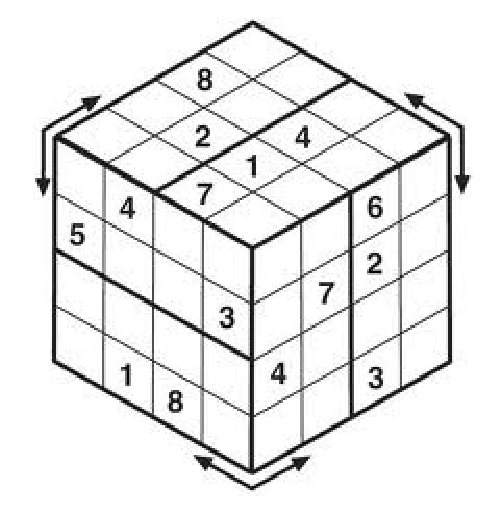
\includegraphics[width=0.3\textwidth]{images}
 \caption{这是一个图片测试例子(中)}
 \label{fig:amss1}
\end{figure}

该页是专门用来测试插入图片的方法,这个方法有很多种,需要自己花点时间来研究学习下,就像表格一样,
下面这只是一个简单的例子。好了,结束。

\subsection{图形位于页面上}
该页是专门用来测试插入图片的方法,这个方法有很多种,需要自己花点时间来研究学习下,就像表格一样,
下面这只是一个简单的例子。好了,结束。该页是专门用来测试插入图片的方法,这个方法有很多种,需要自己花点时间来研究学习下,就像表格一样,
下面这只是一个简单的例子。好了,结束。

\begin{figure}[t]
 \centering
 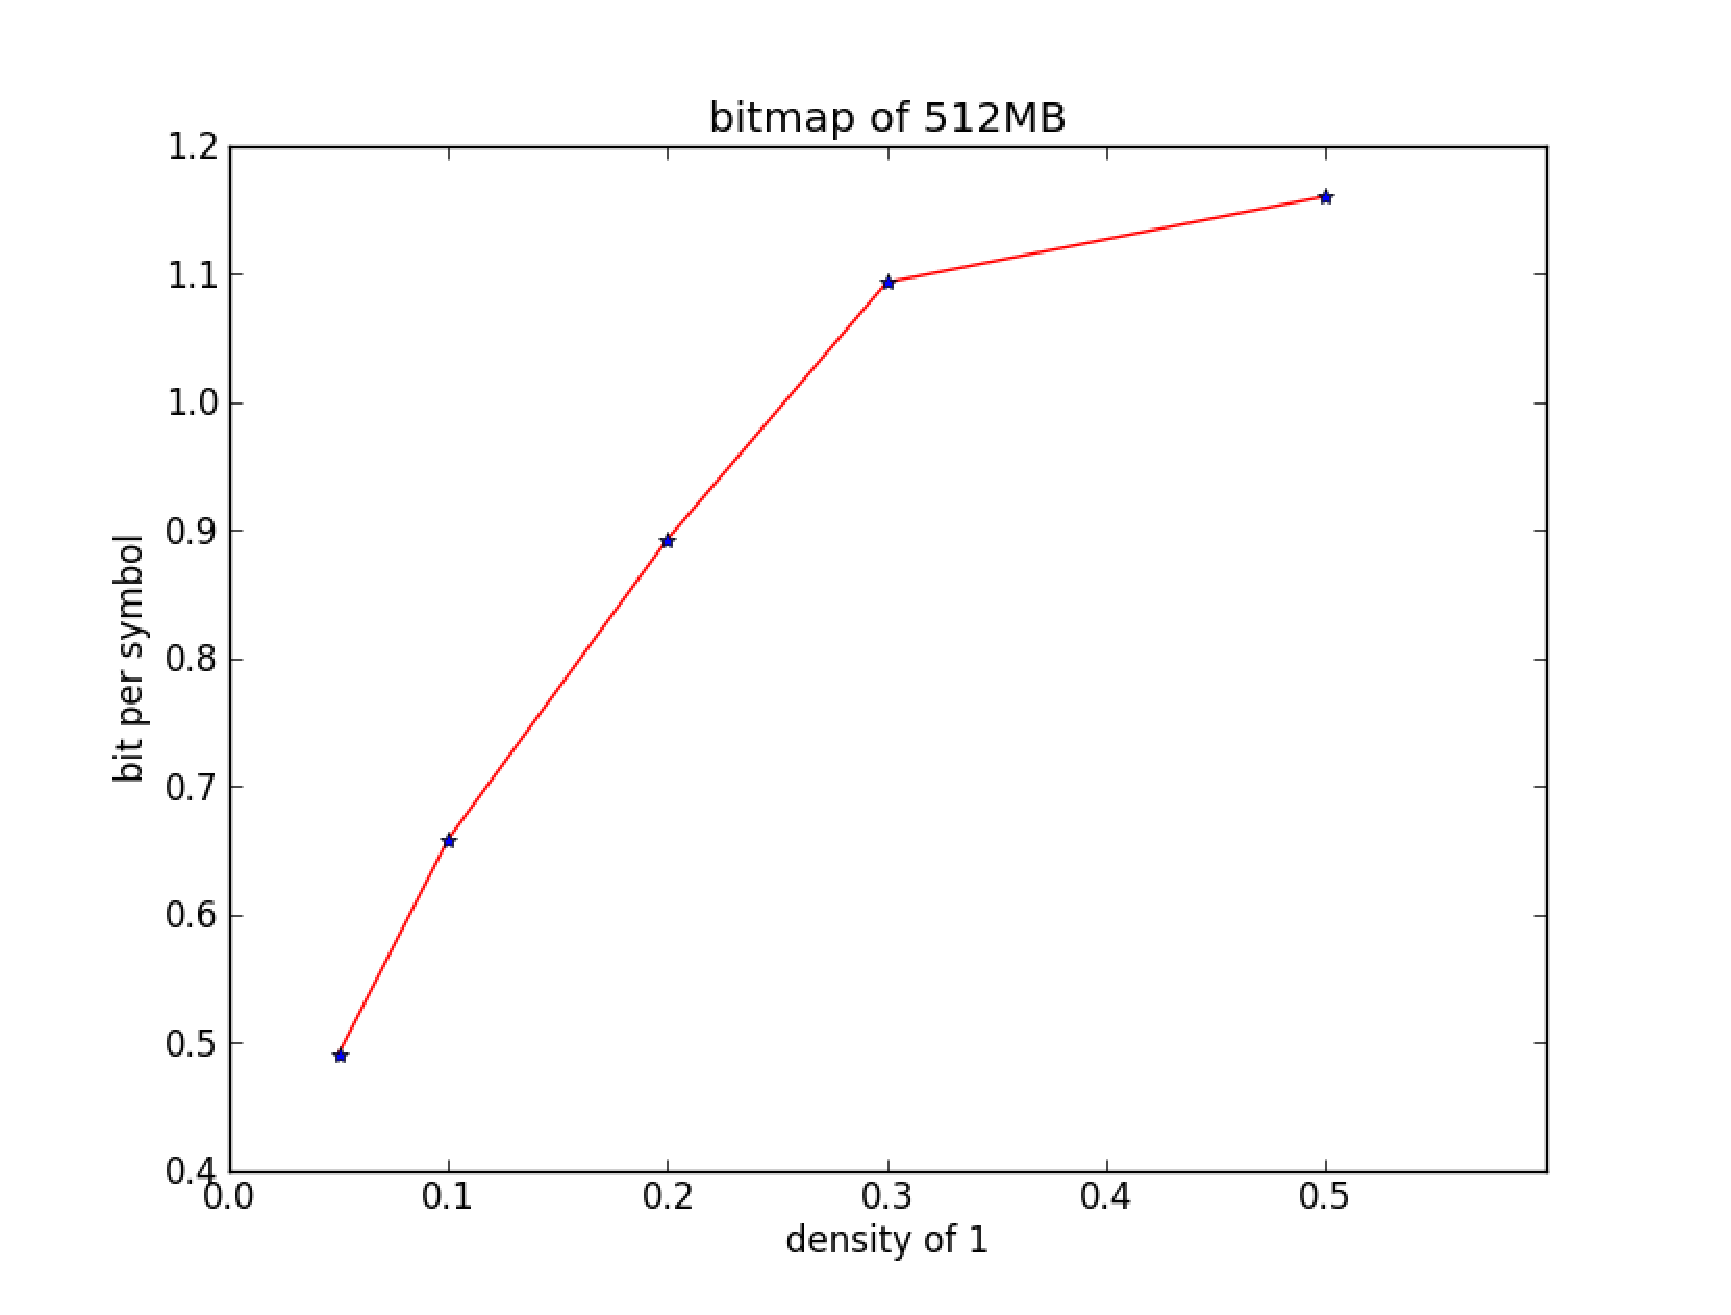
\includegraphics[width=0.3\textwidth]{rrr}
 \caption{这是一个图片测试例子(上)}
 \label{fig:amss2}
\end{figure}

该页是专门用来测试插入图片的方法,这个方法有很多种,需要自己花点时间来研究学习下,就像表格一样,
下面这只是一个简单的例子。该页是专门用来测试插入图片的方法,这个方法有很多种,需要自己花点时间
来研究学习下,就像表格一样,下面这只是一个简单的例子。该页是专门用来测试插入图片的方法,这个方法
有很多种,需要自己花点时间来研究学习下,就像表格一样,下面这只是一个简单的例子。

\subsection{图形位于页面下}
该页是专门用来测试插入图片的方法,这个方法有很多种,需要自己花点时间来研究学习下,就像表格一样,
下面这只是一个简单的例子。

\begin{figure}[b]
 \centering
 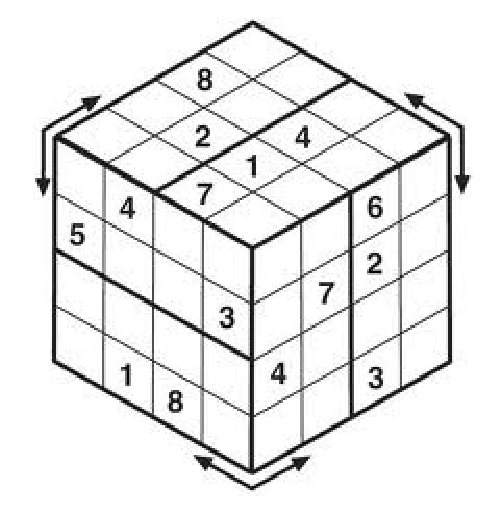
\includegraphics[width=0.3\textwidth]{images}
 \caption{这是一个图片测试例子(下)}
 \label{fig:amss3}
\end{figure}


该页是专门用来测试插入图片的方法,这个方法有很多种,需要自己花点时间来研究学习下,就像表格一样,
下面这只是一个简单的例子。该页是专门用来测试插入图片的方法,这个方法有很多种,需要自己花点时间
来研究学习下,就像表格一样,下面这只是一个简单的例子。

该页是专门用来测试插入图片的方法,这个方法
有很多种,需要自己花点时间来研究学习下,就像表格一样,下面这只是一个简单的例子。该页是专门用来测
试插入图片的方法,这个方法有很多种,需要自己花点时间来研究学习下,就像表格一样,
下面这只是一个简单的例子。

该页是专门用来测试插入图片的方法,这个方法有很多种,需要自己花点时间来研究学习下,就像表格一样,
下面这只是一个简单的例子。该页是专门用来测试插入图片的方法,这个方法有很多种,需要自己花点时间
来研究学习下,就像表格一样,下面这只是一个简单的例子。

该页是专门用来测试插入图片的方法,这个方法
有很多种,需要自己花点时间来研究学习下,就像表格一样,下面这只是一个简单的例子。该页是专门用来测
试插入图片的方法,这个方法有很多种,需要自己花点时间来研究学习下,就像表格一样,
下面这只是一个简单的例子。

该页是专门用来测试插入图片的方法,这个方法有很多种,需要自己花点时间来研究学习下,就像表格一样,
下面这只是一个简单的例子。该页是专门用来测试插入图片的方法,这个方法有很多种,需要自己花点时间
来研究学习下,就像表格一样,下面这只是一个简单的例子。该页是专门用来测试插入图片的方法,这个方法
有很多种,需要自己花点时间来研究学习下,就像表格一样,下面这只是一个简单的例子。该页是专门用来测
试插入图片的方法,这个方法有很多种,需要自己花点时间来研究学习下,就像表格一样,
下面这只是一个简单的例子。


    
\chapter{总结与展望}
\label{chap:con}

\subsection{总结}

\subsection{进一步工作}


    \appendix
    
\chapter[本科生毕业设计论文撰写规范]{西安电子科技大学本科生毕业设计论文撰写规范}
\label{chap:requires}
\section{毕业设计(论文)的总体要求}
撰写论文应简明扼要,一般不少于15000字(外语专业可适当减少,但不得少于10000单词,且须全部用外语书写)。

\section{毕业设计(论文)的编写格式}
每一章、节的格式和版面要求整齐划一、层次清楚。其中:
\begin{itemize}
  \item 论文用纸:统一用A4纸,与论文封皮,任务书,工作计划,成绩考核表一致。
  \item 章的标题:如:``摘要''、``目录''、``第一章''、``附录''等,黑体,三号,居中排列。
  \item 节的标题:如:``2.1  认证方案''、``9.5  小结''等,宋体,四号,居中排列。
  \item 正文:中文为宋体,英文为``Times News Roman'',小四号。正文中的图名和表名,宋体,五号。
  \item 页眉:宋体五号,居中排列。左面页眉为论文题目,右面页眉为章次和章标题。页眉底划线的宽度为0.75磅。
  \item 页码:宋体小五号,排在页眉行的最外侧,不加任何修饰。
\end{itemize}

\section{毕业设计(论文)的前置部分}
毕业设计(论文)的前置部分包括封面、中英文摘要、目录等。
\subsection{封面及打印格式}
\begin{itemize}
  \item 学号:按照学校的统一编号,在右上角正确打印自己的学号,宋体,小四号,加粗。
  \item 题目:题目应和任务书的题目一致,黑体,三号。
  \item 学院、专业、班级、学生姓名和导师姓名职称等内容,宋体,小三号,居中排列。
\end{itemize}

\subsection{中英文摘要及关键词}
摘要是关于论文的内容不加注释和评论的简短陈述,具有独立性和自含性。它主要是
简要说明研究工作的目的、方法、结果和结论,重点说明本论文的成果和新见解。关键词
是为了文献标引工作从论文中选取出来用以表示全文主题内容信息的术语。
\begin{enumerate}
  \item 中文摘要,宋体小四号,一般为300字;英文摘要,``Times News Roman''字
体,小四号,一般为300个实词。摘要中不宜出现公式、非公用的符号、术语等。
  \item 每篇论文选取3 \~{} 5个关键词,中文为黑体小四号,英文为``Times News Roman''字体加粗,小四号。关键词排列在摘要的左下方一行,起始格式为:``\textbf{关键词}:
      ''和``\textbf{Keyword:}''。具体的各个关键词以均匀间隔排列,之间不加任何分隔符号。
\end{enumerate}

\section{目录}
按照论文的章、节、附录等前后顺序,编写序号、名称和页码。目录页排在中英文摘要之后,主体部分必
须另页右面开始,全文以右页为单页页码。

\section{毕业设计(论文)的主体部分}
毕业设计(论文)的主体部分包括引言(绪论)、正文、结论、结束语、致谢、参考文献。
\subsection{绪论}
作为论文的开端,简要说明作者所做工作的目的、范围、国内外进展情况、前人研究成果、
本人的设想、研究方法等。
\subsection{正文} 为毕业设计(论文)的核心部分,包括理论分析、数据资料、实验方法、结果、本人的论点和结
论等内容,还要附有各种有关的图表、照片、公式等。要求理论正确、逻辑清楚、层次分明、文字流畅、数据真实可
靠,公式推导和计算结果无误,图表绘制要少而精。
\begin{description}
  \item[图] 包括曲线图、示意图、流程图、框图等。图序号一律用阿拉伯数字分章依序编码,如:图1.3、图2.11。每一图应有简短确切的
      图名,连同图序号置于图的正下方。图中坐标上标注的符号和缩略词必须与正文中一致。
  \item[表] 包括分类项目和数据,一般要求分类项目由左至右横排,数据从上到下竖列。分类项目横排中必须标明符号或单位,竖列的数据栏中不宜出现``同上'' 、``同左''等类似词语,一律填写具体的数字或文字。表序号一律用阿拉伯数字分章依序编码,如:表2.5、表10.3。每一表应有简短确切的题名,
      连同表序号置于表的正上方。
  \item[公式] 正文中的公式、算式、方程式等必须编排序号,序号一律用阿拉伯数字分章依序编码,如:式(3-32)、式(6-21)。对于较长的公式,另行居中横排,只可在符号处(如:+、-、*、/、$<$、 $>$等)转行。公式序号标注于该式所在行(当有续行时,应标注于最后 一行)的最右边。连续性的公式在``=''处排列整齐。大于999的整数或多于三位的小数,一律用半个阿拉伯数字符的小间隔分开;小于1的数应将0置于小数点之前。
  \item[计量单位] 单位名称和符号的书写方式一律采用国际通用符号。
\end{description}

\subsection{结论}
是对主体的最终结论,应准确、完整、精炼。阐述作者创造性工作在本研究领域的地位和作用,对存在的问题和不足应给予客观的说明,也可提出进一步的设想。

\subsection{致谢}
对协助完成论文研究工作的单位和个人表示感谢。

\subsection{参考文献}
在学位论文中引用参考文献时,引出处右上角用方括号标注阿拉伯数字编排的序号(必须与参考文献一致)。参考文献的排列格
式分为:
\begin{description}
  \item[专著类的文献] [序号]  作者 . 专著名称.  版本. 出版地:出版者,出版年. 参考的页码。
  \item[期刊类的文献] 作者 . 文献名. 期刊名称.  年 , 月,  卷(期). 页码。
\end{description}
其中作者采用姓在前、名在后的形式。当作者超过三个时,只著录前三个人,其后
加``等''字即可。

\section{毕业设计(论文)的附录部分}
附录是作为学位论文主体的补充,包括下列内容:
\begin{enumerate}
  \item 正文中过于冗长的公式推导;
  \item 为读者阅读方便所需要的辅助性的数学工作或带有重复性的图表;
  \item 由于过分冗长而不宜在正文中出现的计算机程序清单;
  \item 对于一般读者并非必要阅读,但对本专业同行有参考价值的资料。
  \item 附录编于正文后,与正文连续编页码,每一附录均另页起。
  \item 附录依次用大写正体A,B,C……编序号,黑体,三号。如:附录A。
  \item 附录中的图、表、式、参考文献等与正文分开,用阿拉伯数字另行编序号,注意在数码前冠以附录的
      序码。如:图A1;表B2;式(C-3);文献[D5]。
\end{enumerate}
\section{毕业设计(论文)的打印规格}
论文正文页面和版面的设置规格:论文正文双面打印,为了便于装订、复制,要求每页纸的四周留有足够的空白边缘。以WORD97为例:

页面设置数据为:上3厘米、下2厘米、内侧3厘米、外侧2厘米;装订线 -- 1厘米;页眉  - 2厘米;  页脚 - 1厘米。

版面设置数据为:文字的行间距 - 1. 5倍 ;  公式的行间距 - 1. 5倍字符间距 - 标准;页码数据-对称页边距。

\section{毕业设计(论文)的装订说明}
毕业设计(论文)要求以A4纸的标准,按照下列顺序装订。外文资料翻译原文及译文另册装订,格式参照论文对应内容格式要求。

\begin{enumerate}
  \item 封面
  \item 任务书
  \item 工作计划
  \item 中期检查表
  \item 成绩考核登记表
  \item 中、外论文摘要
  \item 目录
  \item 引言
  \item 论文
  \item 结论
  \item 结束语
  \item 参考文献
  \item 附录
\end{enumerate}












%%----------------- 附件部分 ----------------- %%
    \backmatter
    
\begin{thanks}

毕业论文暂告收尾,这也意味着我在西安电子科技大学的四年的学习生活既将结束。
回首既往,自己一生最宝贵的时光能于这样的校园之中,能在众多学富五车、才华
横溢的老师们的熏陶下度过,实是荣幸之极。在这四年的时间里,我在学习上和思
想上都受益非浅。这除了自身努力外,与各位老师、同学和朋友的关心、支持和鼓
励是分不开的论文的写作是枯燥艰辛而又富有挑战的。

数学是理论界一直探讨的热门话题,老师的谆谆诱导、同学的出谋划策及家长的支持
鼓励,是我坚持完成论文的动力源泉。在此,我特别要感谢我的导师xxx老师。从论文
的选题、文献的采集、框架的设计、结构的布局到最终的论文定稿,从内容到格式,
从标题到标点,她都费尽心血。没有xxx老师的辛勤栽培、孜孜教诲,就没有我论文
的顺利完成。

感谢数学系的各位同学,与他们的交流使我受益颇多。最后要感谢我的家人以及我的
朋友们对我的理解、支持、鼓励和帮助,正是因为有了他们,我所做的一切才更有意
义;也正是因为有了他们,我才有了追求进步的勇气和信心。

时间的仓促及自身专业水平的不足,整篇论文肯定存在尚未发现的缺点和错误。
恳请阅读此篇论文的老师、同学,多予指正,不胜感激!
......

\vskip 18pt

谨把本文献给我最敬爱的父母亲以及所有关心我的人!

\end{thanks}

    %\include{chapter-utf8/bib1}
    \bibliography{reference}

\end{document}



